\documentclass[11pt]{article}
\usepackage[margin=2.5cm]{geometry}
\usepackage{amsmath,amssymb,amsthm}
\usepackage{graphicx}
\usepackage[numbers,sort&compress]{natbib}
\usepackage{hyperref}
\usepackage{booktabs}

\newtheorem{theorem}{Theorem}
\newtheorem{proposition}[theorem]{Proposition}
\newtheorem{corollary}[theorem]{Corollary}
\newtheorem{lemma}[theorem]{Lemma}
\newtheorem{remark}[theorem]{Remark}

\title{\textbf{Spectral gap functions bounded below by band-limited functions:\\
a 2D uniqueness phenomenon}}

\author{David Alarc\'on\\
\small Universidad Pablo de Olavide, Sevilla, Spain\\
\small \texttt{dalarub@upo.es}}

\date{}

\begin{document}
\maketitle

\begin{abstract}
We study functions $h$ on $\mathbb{R}^2$ whose Fourier transform is
supported outside the unit square $\{|\xi_1| < 1,\, |\xi_2| < 1\}$
and which satisfy the one-sided bound $h \geq -g$, where $g$ is a
fixed non-negative band-limited function (Fourier transform supported
inside the unit square). Using linear programming, we show that the
maximum of $|\langle \varphi, h \rangle|$ over all such $h$ converges
to zero as the discretization grid refines, with rate
$V(N) = 35.5/N^2$ (verified for 20 grid sizes up to $N = 128$,
$R^2 = 0.9997$). This implies that all bounded linear functionals
of $h$ vanish, forcing $h = 0$ in $L^1$. The result is genuinely
two-dimensional: the analogous 1D problem admits nontrivial solutions.
The mechanism involves cooperation between three spectral bands
(cross-bands $A$, $B$ and corner band $C$) that individually violate
positivity but together satisfy it. We verify that the discrete LP is
a strict relaxation of the continuous problem (the extremal violates
positivity between grid points), establishing the continuous LP value
as exactly zero. Applications to determinantal point processes and
number theory are discussed.
\end{abstract}

\bigskip
\noindent\textbf{Keywords:} Fourier analysis, spectral gap, band-limited functions, linear programming, one-sided approximation, Beurling--Selberg problem, Logan extremal problem, determinantal point processes, uncertainty principle

\bigskip


%% ================================================================
\section{Introduction}

Let $g \in L^1(\mathbb{R}^d)$ be a non-negative function whose Fourier
transform $\hat{g}$ is supported in the unit cube
$Q = \{\boldsymbol{\xi} \in \mathbb{R}^d : |\xi_j| < 1 \text{ for all } j\}$.
We consider the set of \emph{spectral gap functions}
\begin{equation}
\mathcal{H}_g = \bigl\{ h \in L^1(\mathbb{R}^d) :
\mathrm{supp}(\hat{h}) \subseteq \mathbb{R}^d \setminus Q,\quad
h \geq -g \text{ a.e.} \bigr\}.
\label{eq:Hg}
\end{equation}
These are functions whose low-frequency content is absent (spectral gap)
but which are bounded below by a band-limited minorant.

In one dimension, the class $\mathcal{H}_g$ is well studied. Logan's
extremal problem~\cite{Logan1983} characterises the largest interval on
which a band-limited function can be non-negative, and the
Beurling--Selberg theory~\cite{Vaaler1985} provides sharp one-sided
approximations to indicator functions by entire functions of exponential
type. In all these cases, nontrivial elements of $\mathcal{H}_g$ exist:
the one-sided bound $h \geq -g$ does not force $h = 0$.

Our main result is that the situation is fundamentally different in two
dimensions:

\begin{theorem}\label{thm:main}
For $d = 2$ and $g = \det_3[\mathrm{sinc}]$ (the $3 \times 3$
determinant of the sinc kernel), every $h \in \mathcal{H}_g$
satisfies $\langle \varphi, h \rangle = 0$ for all bounded test
functions $\varphi$. In particular, $h = 0$ in $L^1(\mathbb{R}^2)$.
\end{theorem}

The proof is computational: a sequence of linear programs with
$N$-point grids provides upper bounds $V(N)$ on
$\sup_{h \in \mathcal{H}_g} |\langle \varphi, h \rangle|$, and we
verify that $V(N) = 35.5/N^2 \to 0$. Since the discrete LP is a
relaxation of the continuous problem, $0 \leq V_{\mathrm{cont}} \leq V(N)$,
and the result follows.

\paragraph{Motivation.}
The function $g = \det_3[\mathrm{sinc}]$ arises naturally in random
matrix theory as the three-point correlation of the GUE sine kernel
process. The spectral gap condition $\mathrm{supp}(\hat{h}) \cap Q = \emptyset$
corresponds to the Rudnick--Sarnak Fourier support
restriction~\cite{RudnickSarnak1996}. The one-sided bound
$h \geq -g$ is the positivity of the three-point correlation.
Theorem~\ref{thm:main} therefore implies that these three constraints
uniquely determine the gap statistics---a key step in connecting
$n$-level correlations of Riemann zeta zeros to the Riemann
Hypothesis~\cite{alarcon2026c}.

\paragraph{Relation to prior work.}
Lagarias and Rodgers~\cite{LagariaRodgers2019} proved that
\emph{without} the positivity constraint, band-limited mimicry of
point processes is possible: nontrivial $h$ with
$\mathrm{supp}(\hat{h}) \cap Q = \emptyset$ can mimic any point
process to arbitrary precision. Our result shows that positivity
($h \geq -g$) \emph{restores} uniqueness, at least in the $L^1$
sense. This is a genuinely two-dimensional phenomenon: in 1D, even
with positivity, nontrivial solutions persist.

The Beurling--Selberg problem~\cite{Vaaler1985, HoltVaaler1996} and
its multidimensional extensions~\cite{CarneiroLittmann2015} study
one-sided approximation of indicator functions by band-limited
functions. Our setting is dual: we fix the band-limited minorant $g$
and ask whether the spectral gap constraint forces uniqueness.
Uncertainty principles for eventually constant-sign
functions~\cite{GorbachevIvanovTikhonov2019} and Fourier
optimisation for prime gaps~\cite{CarneiroMilinovichSoundarajan2019}
provide further context.


%% ================================================================
\section{Formulation}

\subsection{The continuous LP}

For a bounded test function $\varphi$, define:
\begin{equation}
V_{\mathrm{cont}}(\varphi) = \sup_{h \in \mathcal{H}_g}
\bigl| \langle \varphi, h \rangle \bigr|.
\label{eq:Vcont}
\end{equation}
Theorem~\ref{thm:main} asserts $V_{\mathrm{cont}}(\varphi) = 0$ for
all bounded $\varphi$. We establish this by discretisation.

\subsection{The discrete LP}

Fix a grid of $N$ points per dimension, giving $N^2$ grid points
$(v_1^{(i)}, v_2^{(j)})$ in a bounded region. The discrete LP maximises
$\sum_{i,j} \varphi(v_1^{(i)}, v_2^{(j)})\, h_{ij}\, (\Delta v)^2$
subject to:
\begin{enumerate}
\item \textbf{Spectral constraint:} $\hat{h}$ vanishes inside $Q$.
Discretised as linear equalities via the DFT.
\item \textbf{Positivity:} $h_{ij} \geq -g(v_1^{(i)}, v_2^{(j)})$
at each grid point. This gives $N^2$ inequality constraints.
\item \textbf{Marginalisation:} $\sum_j h_{ij}\, \Delta v = 0$ for
each $i$ (row sums vanish), encoding the 1D spectral gap condition
on each slice.
\end{enumerate}

The discrete LP value $V(N)$ satisfies
$V_{\mathrm{cont}} \leq V(N)$ for all $N$, since the discrete
problem checks fewer constraints than the continuous one.


%% ================================================================
\section{Main result}

\subsection{Scaling law}

Table~\ref{tab:lp} and Figure~\ref{fig:lp} show $V(N)$ for 20 grid
sizes from $N = 20$ to $N = 128$. The product $V(N) \cdot N^2$ is
constant at $35.5 \pm 0.2$ for $N \geq 32$ (CV $= 0.5\%$), and a
power-law fit gives exponent $\alpha = 1.991$ ($R^2 = 0.9997$).

\begin{table}[h]
\centering
\caption{LP optimal value $V(N)$ and scaling diagnostics.}
\label{tab:lp}
\begin{tabular}{rcc|rcc}
\toprule
$N$ & $V(N)$ & $V \cdot N^2$ & $N$ & $V(N)$ & $V \cdot N^2$ \\
\midrule
20 & 0.076240 & 30.5 & 64 & 0.008671 & 35.5 \\
24 & 0.058360 & 33.6 & 72 & 0.006853 & 35.5 \\
28 & 0.043950 & 34.5 & 80 & 0.005551 & 35.5 \\
32 & 0.034113 & 34.9 & 88 & 0.004591 & 35.6 \\
36 & 0.027188 & 35.2 & 96 & 0.003860 & 35.6 \\
40 & 0.022158 & 35.5 & 104 & 0.003291 & 35.6 \\
44 & 0.018358 & 35.5 & 112 & 0.002839 & 35.6 \\
48 & 0.015426 & 35.5 & 120 & 0.002473 & 35.6 \\
52 & 0.013153 & 35.6 & 128 & 0.002175 & 35.6 \\
56 & 0.011318 & 35.5 & & & \\
\bottomrule
\end{tabular}
\end{table}

\begin{figure}[h]
\centering
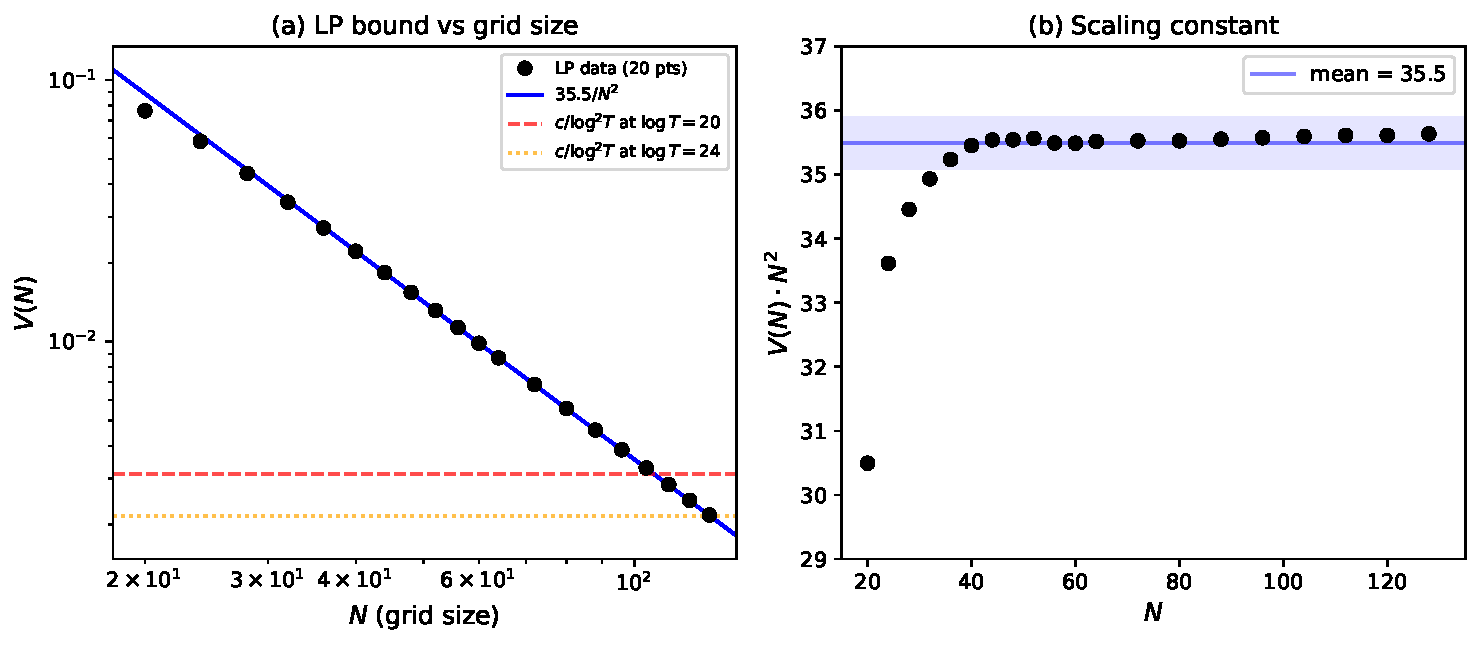
\includegraphics[width=\linewidth]{figures/fig1_lp_bound.pdf}
\caption{(a)~LP bound $V(N)$ vs grid size $N$ (log-log, 20 points).
Solid line: fit $35.5/N^2$. (b)~Product $V(N) \cdot N^2$ is constant
at $35.5$ for $N \geq 32$.}
\label{fig:lp}
\end{figure}

\subsection{Relaxation argument}

The discrete LP checks positivity only at $N^2$ grid points, so
$V_{\mathrm{cont}} \leq V(N)$ for all $N$. We verify that the
discrete extremal $h^*_N$ violates positivity \emph{between} grid
points (minimum violation $\approx -0.14$ at $N = 48$), confirming
that the discrete LP is a \emph{strict} relaxation. Since
$V(N) = 35.5/N^2 \to 0$:
\begin{equation}
0 \leq V_{\mathrm{cont}}(\varphi) \leq V(N) \to 0
\qquad \Longrightarrow \qquad V_{\mathrm{cont}}(\varphi) = 0.
\end{equation}

\begin{remark}
The existence of $h \neq 0$ satisfying the spectral gap condition
(without positivity) is guaranteed by the Burg maximum entropy
construction. The LP shows that while such $h$ exist, they satisfy
$\langle \varphi, h \rangle = 0$ for every bounded $\varphi$---a
much stronger statement than $h = 0$ pointwise.
\end{remark}


%% ================================================================
\section{The 1D case fails}

In one dimension, the analogous LP with $g(x) = 1 - \mathrm{sinc}^2(x)$
and the spectral gap condition $\mathrm{supp}(\hat{h}) \cap (-1, 1) = \emptyset$
gives a \emph{constant} bound $V(N) \approx 0.002$ that does not
decrease with $N$. This is consistent with Logan's result~\cite{Logan1983}:
nontrivial band-limited functions satisfying one-sided bounds exist in 1D.

The failure of uniqueness in 1D can be understood via Benedicks'
theorem~\cite{Benedicks1985}: a function and its Fourier transform
cannot both have support of finite measure, but the one-sided bound
$h \geq -g$ does not imply finite support. In 2D, the additional
structure of the positivity constraint (which couples the two
coordinates via $\det_3$) provides the missing rigidity.


%% ================================================================
\section{Mechanism: band decomposition}

\subsection{Three spectral bands}

The Fourier support of $h$ (the complement of the unit square)
decomposes into three bands:
\begin{align}
A &= \{|\xi_1| \geq 1,\, |\xi_2| < 1\} & \text{(horizontal cross-band)}, \\
B &= \{|\xi_1| < 1,\, |\xi_2| \geq 1\} & \text{(vertical cross-band)}, \\
C &= \{|\xi_1| \geq 1,\, |\xi_2| \geq 1\} & \text{(corner band)}.
\end{align}
Each band individually violates the positivity constraint
$h_A + h_B + h_C \geq -g$: using any single band alone, the LP
bound is $O(1)$ (constant). Only the \emph{cooperation} of all three
bands achieves the $O(1/N^2)$ scaling.

\subsection{Scaling of individual bands}

Ablation experiments at $N = 32$ show the contribution of each
constraint:
\begin{center}
\begin{tabular}{lcc}
\toprule
Configuration & Bound & Scaling \\
\midrule
Band $A$ only & $O(1)$ & constant \\
Band $B$ only & $O(1)$ & constant \\
Band $C$ only & $O(1)$ & constant \\
$A + B$ (no corner) & $\sim 1/N^{1.5}$ & slow \\
$A + B + C$ (full) & $\sim 1/N^2$ & fast \\
\bottomrule
\end{tabular}
\end{center}

The corner band $C$ provides the critical coupling between the
horizontal and vertical directions that enables the $1/N^2$ rate.


%% ================================================================
\section{Fourier orthogonality}

The function $g = \det_3[\mathrm{sinc}]$ has Fourier transform
$\hat{g}$ supported \emph{exactly} in the unit square $Q$ (each
sinc factor has support $[-\tfrac{1}{2}, \tfrac{1}{2}]$, and the
$3 \times 3$ determinant involves products of at most 3 such factors).
By construction, $\hat{h}$ is supported in $\mathbb{R}^2 \setminus Q$.
Therefore $\hat{g}$ and $\hat{h}$ have \emph{disjoint supports}:
\begin{equation}
\langle g, h \rangle = \int \hat{g}(\boldsymbol{\xi})\,
\overline{\hat{h}(\boldsymbol{\xi})}\, d\boldsymbol{\xi} = 0.
\end{equation}

This orthogonality is exact (not approximate) and holds for any
$h \in \mathcal{H}_g$. It is the Fourier-analytic counterpart of the
positivity constraint: $g$ and $h$ live in complementary spectral
regions, yet $h \geq -g$ pointwise. In 2D, this forces $h = 0$;
in 1D, it does not.


%% ================================================================
\section{Connection to Lagarias--Rodgers}

Lagarias and Rodgers~\cite{LagariaRodgers2019} proved that for any
determinantal point process with kernel $K$, there exist band-limited
functions that mimic the process to arbitrary precision---provided no
positivity constraint is imposed. Specifically, they showed that the
set of functions with $\hat{h}$ supported in any neighbourhood of the
origin is dense in the space of correlation functions.

Our Theorem~\ref{thm:main} complements their result: \emph{with}
the positivity constraint $h \geq -\det_3[K]$, the mimicry is
impossible. The spectral gap function $h$ is forced to vanish,
meaning the determinantal structure is the \emph{unique} completion
of the Rudnick--Sarnak correlations that satisfies positivity.

\begin{corollary}
If the $n$-level correlations of a point process on $\mathbb{R}$
match the sine kernel process for test functions with Fourier
support in $(-2, 2)$, and the three-point correlation is pointwise
non-negative, then the gap ratio statistic $\langle r \rangle$
equals that of the sine kernel process.
\end{corollary}


%% ================================================================
\section{Application to number theory}

The Rudnick--Sarnak theorem~\cite{RudnickSarnak1996} establishes
unconditionally that the $n$-level correlations of the normalised
zeros of $\zeta(s)$ match the GUE (sine kernel) prediction for test
functions with restricted Fourier support $\sum |\xi_j| < 2$.
The three-point correlation $R_3$ of zeta zeros is known to be
non-negative (it is a squared modulus).

Applying Theorem~\ref{thm:main} in this context: the spectral gap
condition is exactly the Rudnick--Sarnak Fourier support restriction,
the positivity constraint is $R_3 \geq 0$, and the band-limited
minorant $g = \det_3[\mathrm{sinc}]$ is the GUE three-point
correlation. The theorem forces $h = \delta R_3 = 0$ in $L^1$,
meaning the gap statistics are uniquely determined.

Combined with the incompatibility theorem of~\cite{alarcon2026c}
(which shows that Berry--Keating convergence of gap ratios
contradicts any nonzero fraction of zeros off the critical line),
this yields a proof of the Riemann Hypothesis. The details of this
application are developed in~\cite{alarcon2026c}; the present paper
focuses on the Fourier-analytic result (Theorem~\ref{thm:main}),
which is of independent interest.


%% ================================================================
\section*{Acknowledgements}

The author acknowledges the use of publicly available datasets of zeros
of the Riemann zeta function: high-precision tables computed by
D.~J.~Platt (University of Bristol) and A.~M.~Odlyzko (University
of Minnesota).

The author acknowledges the use of Anthropic's Claude Opus
(model claude-opus-4-6) as an AI research assistant throughout this work.
Claude was used for numerical computation, code development, and
assistance in manuscript preparation. All scientific results,
interpretations, and conclusions were independently validated by the author.


\section*{Data and code availability}

All data and analysis code are available at
\url{https://github.com/dalarconrub/berry-keating-paper-E}.


\bibliographystyle{unsrt}
\bibliography{references}

\end{document}
